\chapter{Experimientos realizados}
\label{cap:resultados}

Como se ha mostrado hasta ahora, hemos desarrollado un sistema capaz de registrar la información de una serie de sensores y crear un fichero con esa información. Cuando se incia el planteamiento de este proyecto, el paso final del mismo es implementar el sistema en una linea de extrusión industrial sin embargo a la hora de implementar el funcionamiento del mismo, la empresa PELS no puede ceder una de sus líneas de extrusión para la puesta en marcha del sistema debido a la planificación de la producción; se adquiere una extrusora de laboratorio pero los plazos de entregan se alargan y no se tiene acceso a ella a la hora de validar el sistema.\\

Por estos motivos se decide hacer uso de una maqueta de extrusora de filamento para poder comprobar como con el sistema diseñado podemos realizar un estudio avanzado de los problemas que tenemos a la hora de fabricar filamento. De esta manera, podremos validar nuestro sistema y adquirir la experiencia necesaria para cuando el sistema se implemente en una línea de extrusión industrial. \\

A continuación vamos a ver distintos ensayos que se han realizado con el sistema. El objetivo de estos ensayos es demostrar que nuestro sistema es válido para registrar la información que le indiquemos y su posterior análisis. También se abre una investigación sobre la influencia de distintos tipos de regulador sobre el tamaño del diámetro final (lazo de control), a pesar de que no es el objetivo principal del proyecto si es un objetivo secundario que ha surgido con la realización del mismo.

\section{Validación del sistema sin tractora}
\label{sec:FSB}

Como primera aproximación e intentando asemejar el esquema de producción vista en el capítulo \ref{cap:descrip} se va a seguir el esquema mostrado en la Figura \ref{fig:esquemap_FSB}.

\begin{figure}[H]
    \centering
    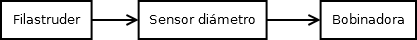
\includegraphics[width=0.6\textwidth]{images/producciones/Diagram1.png}
    \caption[Esquema de producción sin tractora.]{Esquema de producción sin tractora. Se tienen los elementos: Extrusora, sensor de diámetro y bobinadora.}
    \label{fig:esquemap_FSB}
\end{figure}

La boquilla de la filastruder es de 3mm. De esta manera se tiene margen suficiente para regular el filamento aplicando una fuerza de tracción según sale de la extrusora y se va enfriando. A la hora de trabajar con una técnica de conformado como es ésta, es muy importante que la velocidad de salida sea lo más constante posible y también hay que tener en cuenta que se producen cambios en el material tanto de tamaño como de forma según sale de la extrusora \cite{tecno_polimeros}. Tres de estos cambios que afectan al material son: 

\begin{itemize}
	\item {\textbf{Tensionado}: El material es recogido por sistemas de almacenamiento consistentes en rodillos que aplican una tensión. Esto hace que el tamaño del material varíe en función de esa tensión. Nos ayudaremos de esta característica para intentar regular el diámetro final del filamento. El tamaño del diámetro tendrá una relación inversamente proporcional a la velocidad.}
	\item {\textbf{Relajación}: Dentro de la extrusora el material soporta esfuerzos normales y al salir por la boquilla se relaja. Esta relajación será mayor, en función del gradiente de temperatura que haya entre la boquila y el ambiente. La Figura \ref{fig:prod_relajacion} muestra un ejemplo de la deformación sufrida por el material.
		\begin{figure}[H]
	        \centering
	        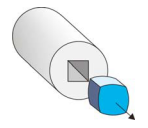
\includegraphics[width=0.2\textwidth]{images/producciones/relajacion.png}
	        \caption[Cambio de tamaño debido a la relajación del material.]{Cambio de tamaño debido a la relajación del material. Fuente \cite{tecno_polimeros}}
	        \label{fig:prod_relajacion}
		\end{figure}
	}
	\item {\textbf{Enfriamiento}: A medida que el material se va enfriando, se va generando una contracción en el perfil del mismo. Está contraccion depende de la velocidad de enfriamiento del material. Por ello, no habrá la misma contracción en una zona gruesa donde haya más material, que en una fina. La Figura \ref{fig:prod_contraccion} muestra un ejemplo de la deformación sufrida por el material.
		\begin{figure}[H]
	        \centering
	        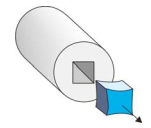
\includegraphics[width=0.2\textwidth]{images/producciones/contraccion.png}
	        \caption[Cambio de tamaño debido a la contraccion del material.]{Cambio de tamaño debido a la contraccion del material. Fuente \cite{tecno_polimeros}}
	        \label{fig:prod_contraccion}
		\end{figure}
	}
\end{itemize}

\subsection{Condiciones del ensayo}

Vamos a comprobar el funcionamiento del sistema con el control de regulación de la propia filawinder, en la que intenta mantener el filamento en una determinada altura y en función de esa altura, aplicar más o menos velocidad de bobinado. Para este primer ensayo se usarán todos los pellets reciclados como materia prima, no se mezclará con PLA transparente, para así ver si el funcionamiento de la filastruder es el correcto.\\

Una vez llegado a la consigna de temperatura de 150ºC se comienza a extruir PLA reciclado y se almacena en la bobina. A simple vista, se ve que la velocidad mínima de bobinado hace que el filamento salga demasiado delgado y se generan demasiadas tensiones en el bobinado del mismo. No obstante, analizaremos los resultados obtenidos. Para el análisis del fihero CSV generado, se usará la herramienta IPython con las librerias, Numpy y Scypi, con los que de manera rápida obtendremos unas conclusiones.\\

Las condiciones iniciales del ensayo son:

    \begin{itemize}
        \item {Duración: 30 min}
        \item {Establecer una temperatura de 135ºC en el extrusor.}
        \item {Llenar la tolva que incluye de serie la extrusora con 42gr de pellets reciclados.}
        \item {Extruir filamento registrando los datos para su posterior análisis.}
    \end{itemize}

\subsection{Análisis de los resultados obtenidos}

Las medidas obtenidas en el ensayo se muestran en la Tabla \ref{tab:result1}, así como en las Figuras \ref{fig:prod_ejes} y \ref{fig:prod_boxplot}.

\begin{table}[H]
	\centering
	\begin{tabular}{ccc}
		{\bf } & {\bf Diámetro X} & {\bf Diámetro Y} \\ \hline
		Muestras & 1110.000000 & 1110.000000 \\
		Media (mm) & 1.17 & 0.91 \\
		Desviación estandar & 0.39 & 0.51 \\
		Mínimo (mm) & 0.01 & 0.00 \\
		Máximo (mm) & 1.92 & 1.74
	\end{tabular}
	\caption[Resultados obtenidos con un sistema sin tractora.]{Resultados obtenidos con un sistema sin tractora.}
	\label{tab:result1}
\end{table}

Cómo podemos comprobar obtenemos una media aritmética de filamento de $ \bar{x} = 1.17mm $  mm con una desviación estandar $\sigma = 0.39$. Representando las medidas de los ejes X e Y podemos comprobar que el resultado no es el deseado:

\begin{figure}[H]
	\centering
	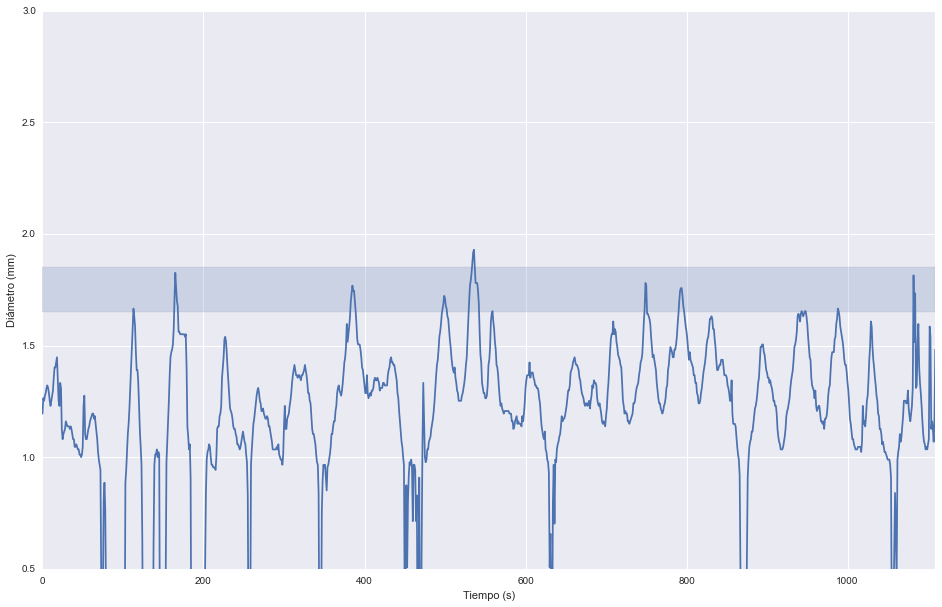
\includegraphics[width=0.99\textwidth]{images/producciones/16062015/output_9_1.png}
	\caption[Representación de las medidas del diámetro de los ejes X e Y.]{Representación de las medidas del diámetro de los ejes X e Y. En el gráfico se muestra una banda de tolerancia, en las que el diámetro filamento se da por válido.}
	\label{fig:prod_ejes}
\end{figure}

Sólo un pequeño número de muestras están por dentro de los márgenes de calidad establecidos por BQ (Max = 1.85mm ; Min = 1.65mm). Además, si representamos los datos en un diagráma de cajas (ver Figura \ref{fig:prod_boxplot}), vemos que hay mucha variación entre los dos ejes.
\begin{figure}[H]
    \centering
    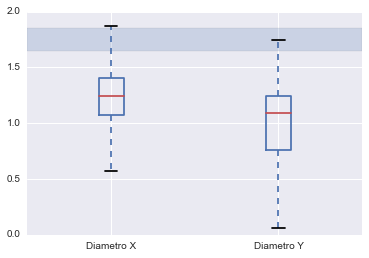
\includegraphics[width=0.5\textwidth]{images/producciones/16062015/output_10_1.png}
    \caption{Diagrama de cajas de las medidas de los ejes X e Y.}
    \label{fig:prod_boxplot}
\end{figure}

Después de los resultados obtenidos en el experimento, descartamos que con este esquema de producción y los materiales disponibles, lleguemos a regular el diámetro de salida de una forma óptima, por tanto se trata de obtener otro esquema de producción para ganarantizar mejores resultados.

\section{Validación del sistema con tractora}
\label{sec:FST}

En una de las pruebas de extrusión de filamento, se va estirando a mano según va saliendo de la filastruder y se comprueba que, traccionando del hilo a una distancia cercana de la boquilla y una vez enfriado, se puede llegar a regular el diámetro final. Por ello se diseña un sistema capaz de traccionar el filamento a medida que es extruido, para comproboar si es posible obtener un filamento con mejor calidad.

\begin{figure}[H]
    \centering
    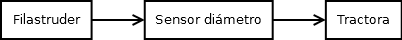
\includegraphics[width=0.6\textwidth]{images/producciones/Diagram2.png}
    \caption[Esquema de producción con tractora.]{Esquema de producción con tractora. Se tienen los elementos: Extrusora, sensor de diámetro, tractora y bobinadora.}
    \label{fig:esquemap_FST}
\end{figure}

Con el conocimiento adquirido al diseñar la peletizadora (ver Anexo \ref{ane:peletizadora}), se diseña una unidad tractora que irá colocada después de la filastruder, la cual, deberá ir traccionando del filamento independientemente del diámetro del mismo. Así mismo, deberemos ser capaces de regular la velocidad de una forma más precisa que como lo hicimos con la peletizadora. En el Anexo \ref{ane:tractora} se detalla el proceso seguido al diseñar la tractora.\\

Una vez se tiene un primer prototipo de la tractora, podemos instalarla en la maqueta (ver Figura \ref{fig:montaje_final}).

\begin{figure}[H]
    \centering
    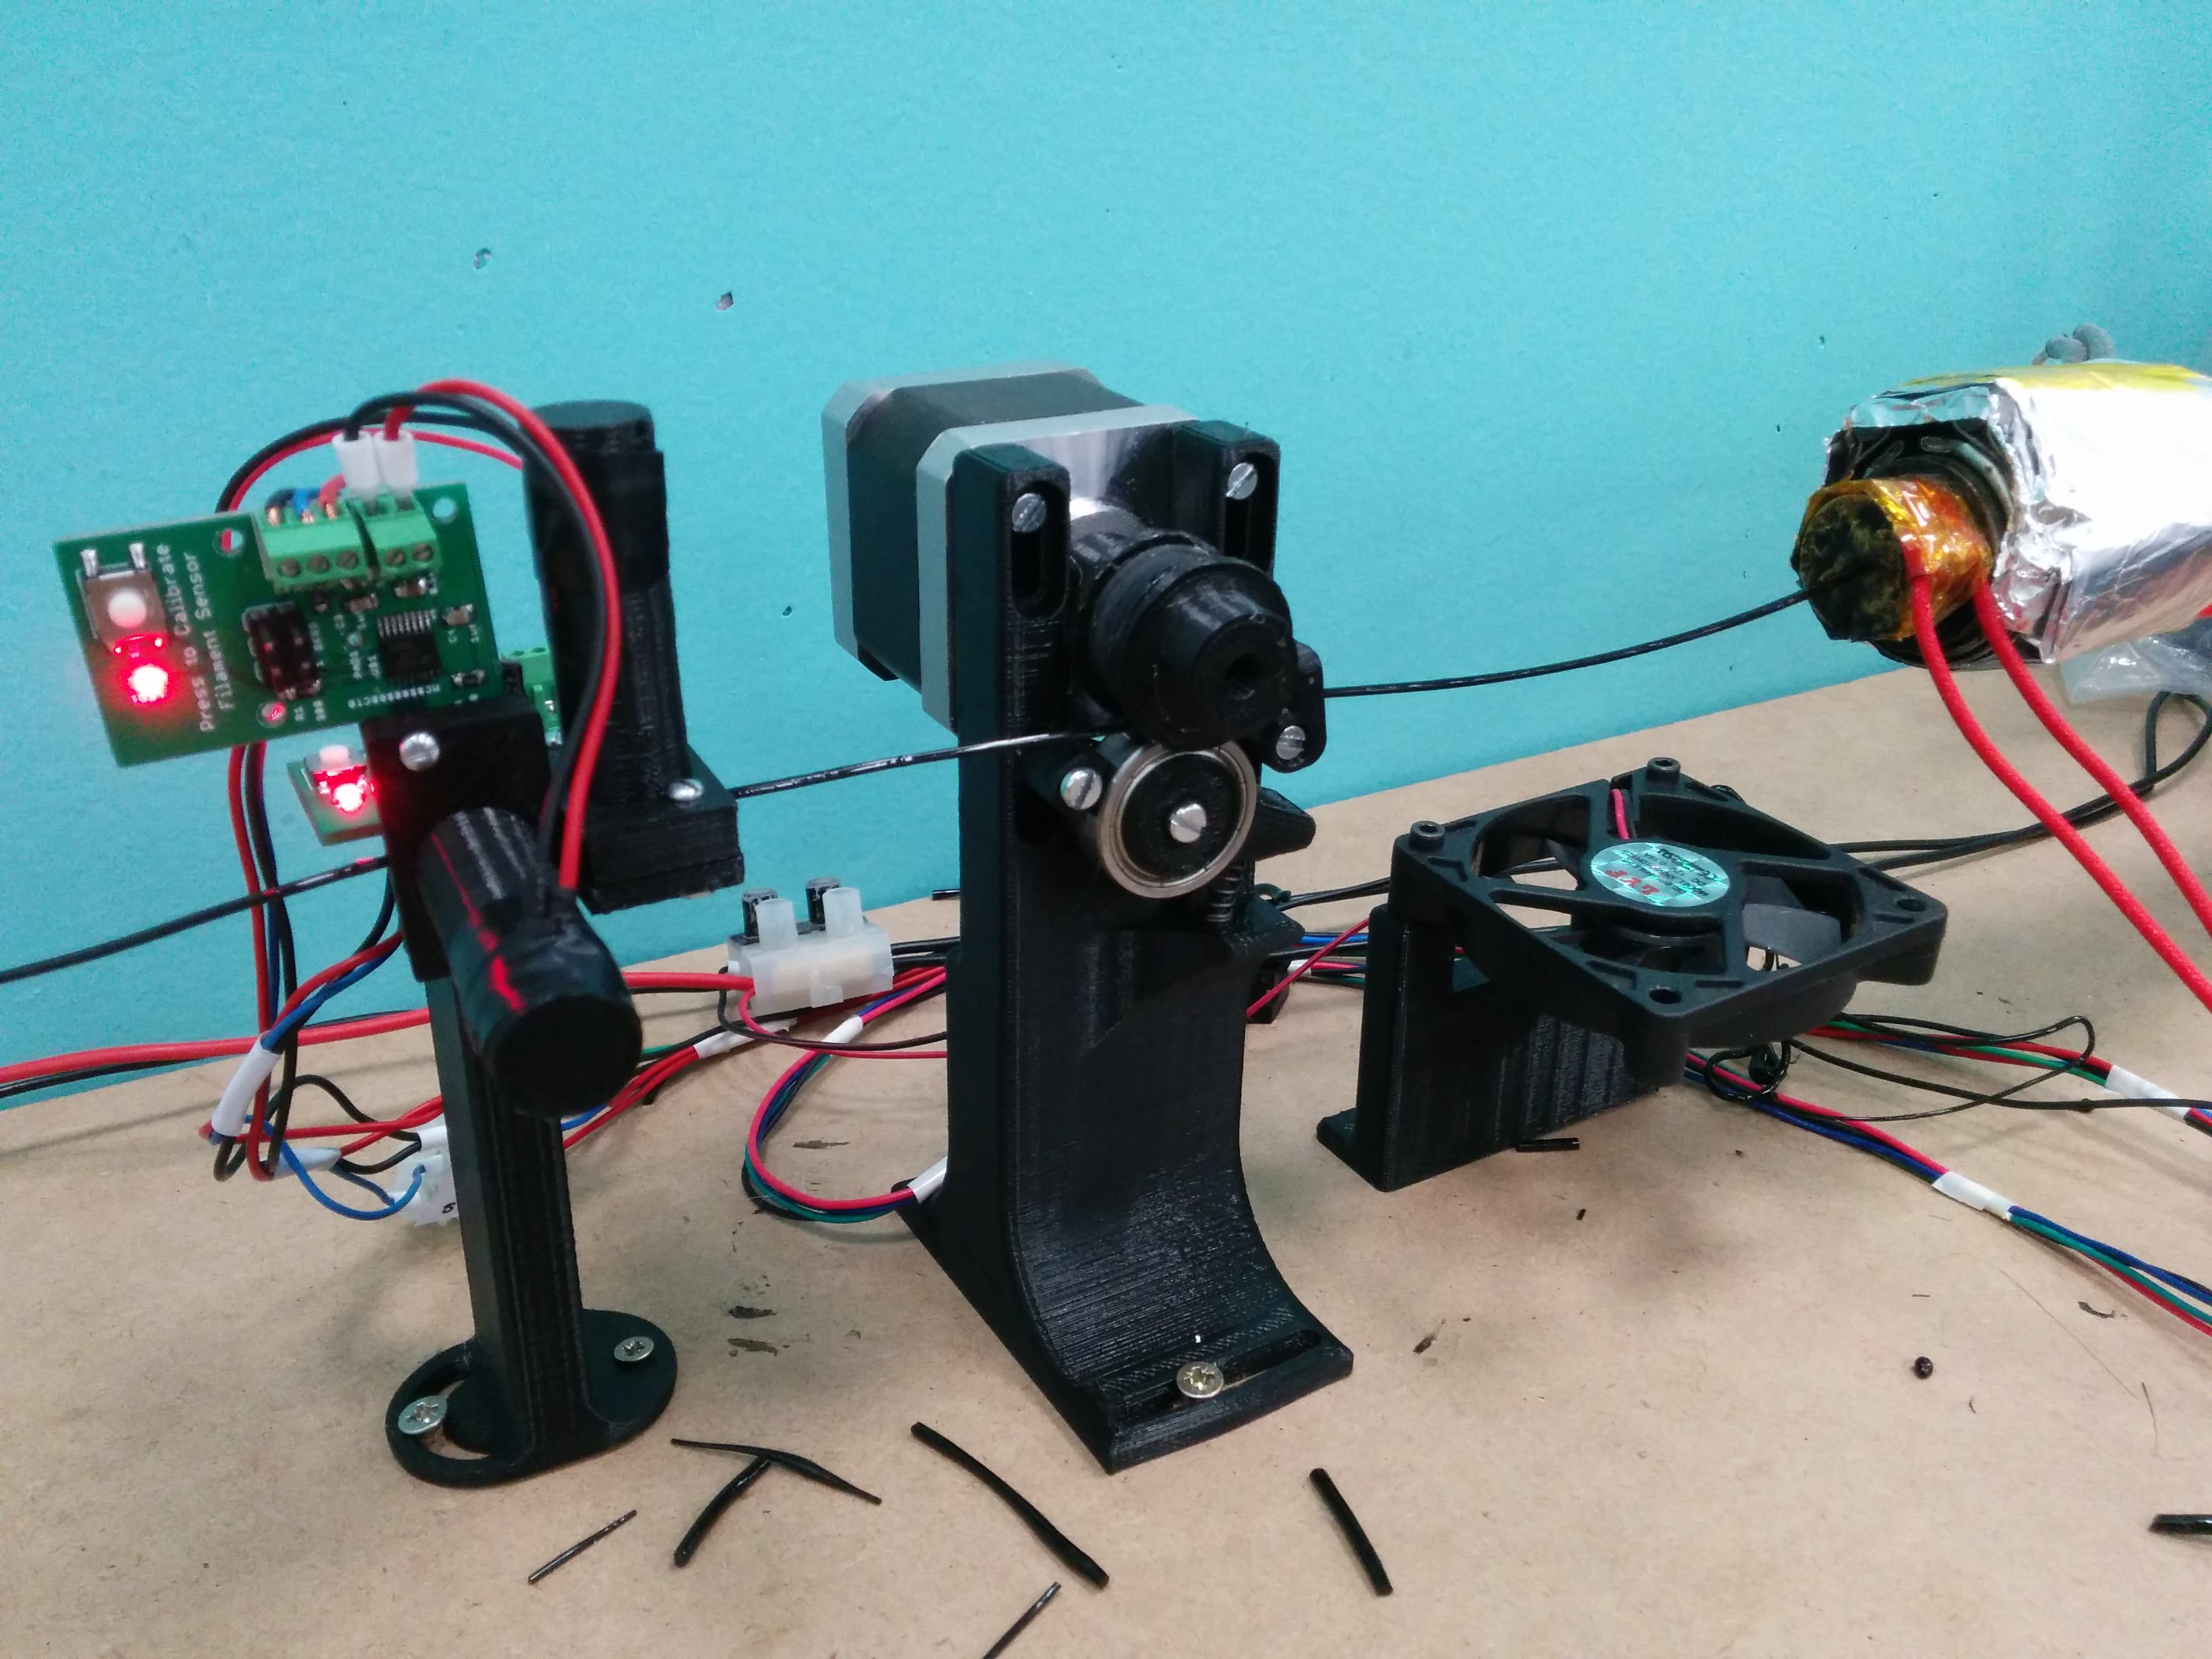
\includegraphics[width=0.6\textwidth]{images/producciones/tractora/IMG_20150709_130326.jpg}
    \caption[Montaje final del sistema con tractora.]{Montaje final del sistema con tractora. (1) Filastruder. (2) Sistema de enfriamiento del filamento. (3) Unidad tractora. (4) Sensor de diámetro.}
    \label{fig:montaje_final}
\end{figure}

\subsection{Condiciones del ensayo}

Usando pellets reciclados y asi confirmar que son válidos para extruir, se realiza una producción de filamento, para comprobar que el diseño de la tractora es el correcto. El ensayo realizado consiste en:

\begin{itemize}
    \item {Duración: 5min}
    \item{Establecer una temperatura de 135ºC en el extrusor.}
    \item{Llenar la tolva que incluye de serie la extrusora con 42gr de pellets reciclados.}
    \item{Extruir filamento registrando los datos para su posterior análisis.}
    \item{Cambiar la velocidad de tracción para comprobar la relación final en el diámetro. Se establecera una velocidad de 1RPM y 3RPM}
\end{itemize}

Durante seis minutos  de producción, el filamento empieza a aumentar el diámetro, provocando que este no pueda pasar a través del sensor de diámetro parando la producción, sin embargo podemos estudiar los datos obtenidos.


\subsection{Análisis de los resultados obtenidos}
Tras el ensayo, los resultados obtenidos son los siguientes:

\begin{table}[H]
    \centering
    \begin{tabular}{cc}
                   & Diámetro X \\ \hline
        Muestras    & 203        \\
        Media (mm) & 1.59       \\
        Desviación estandar & 0.25\\
        Mínimo (mm)   & 1.08       \\
        Máximo (mm)   & 2.19      
    \end{tabular}
    \caption{Resultados obtenidos en un sistema con tractora.}
    \label{tab:20007105-dat}
\end{table}

En la Figura \ref{fig:2007105-graf} vemos los datos obtenidos del diámetro del eje X. Se puede observar que hay una variación muy pronunciada al tener una velocidad de tracción constante, esto es un problema en el diseño de la filastruder ya que, a una velocidad de tracción constante, el diámetro debería serlo también.

\begin{figure}[H]
    \centering
    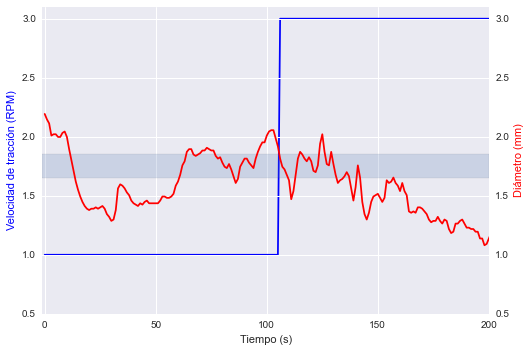
\includegraphics[width=0.99\textwidth]{images/producciones/20072015/output_8_0.png}
    \caption[Gráfica con la relación entre la velocidad de tracción y el diámetro final.]{Gráfica con la relación entre la velocidad de tracción y el diámetro final.}
    \label{fig:2007105-graf}
\end{figure}

 Durante el ensayo, se ha percibido que la extrusión no es constante, por ello, pensamos que el funcionamiento de la filastruder, que a simple vista parecía correcto, no puede llegar a proporcionarnos los resultados que necesitamos. Para comprobar esto, instalamos un encoder mediante un imán, un sensor de efecto hall y un arduino a la filastruder, para cercionarnos de que la velocidad es constante.

\begin{figure}[H]
    \centering
    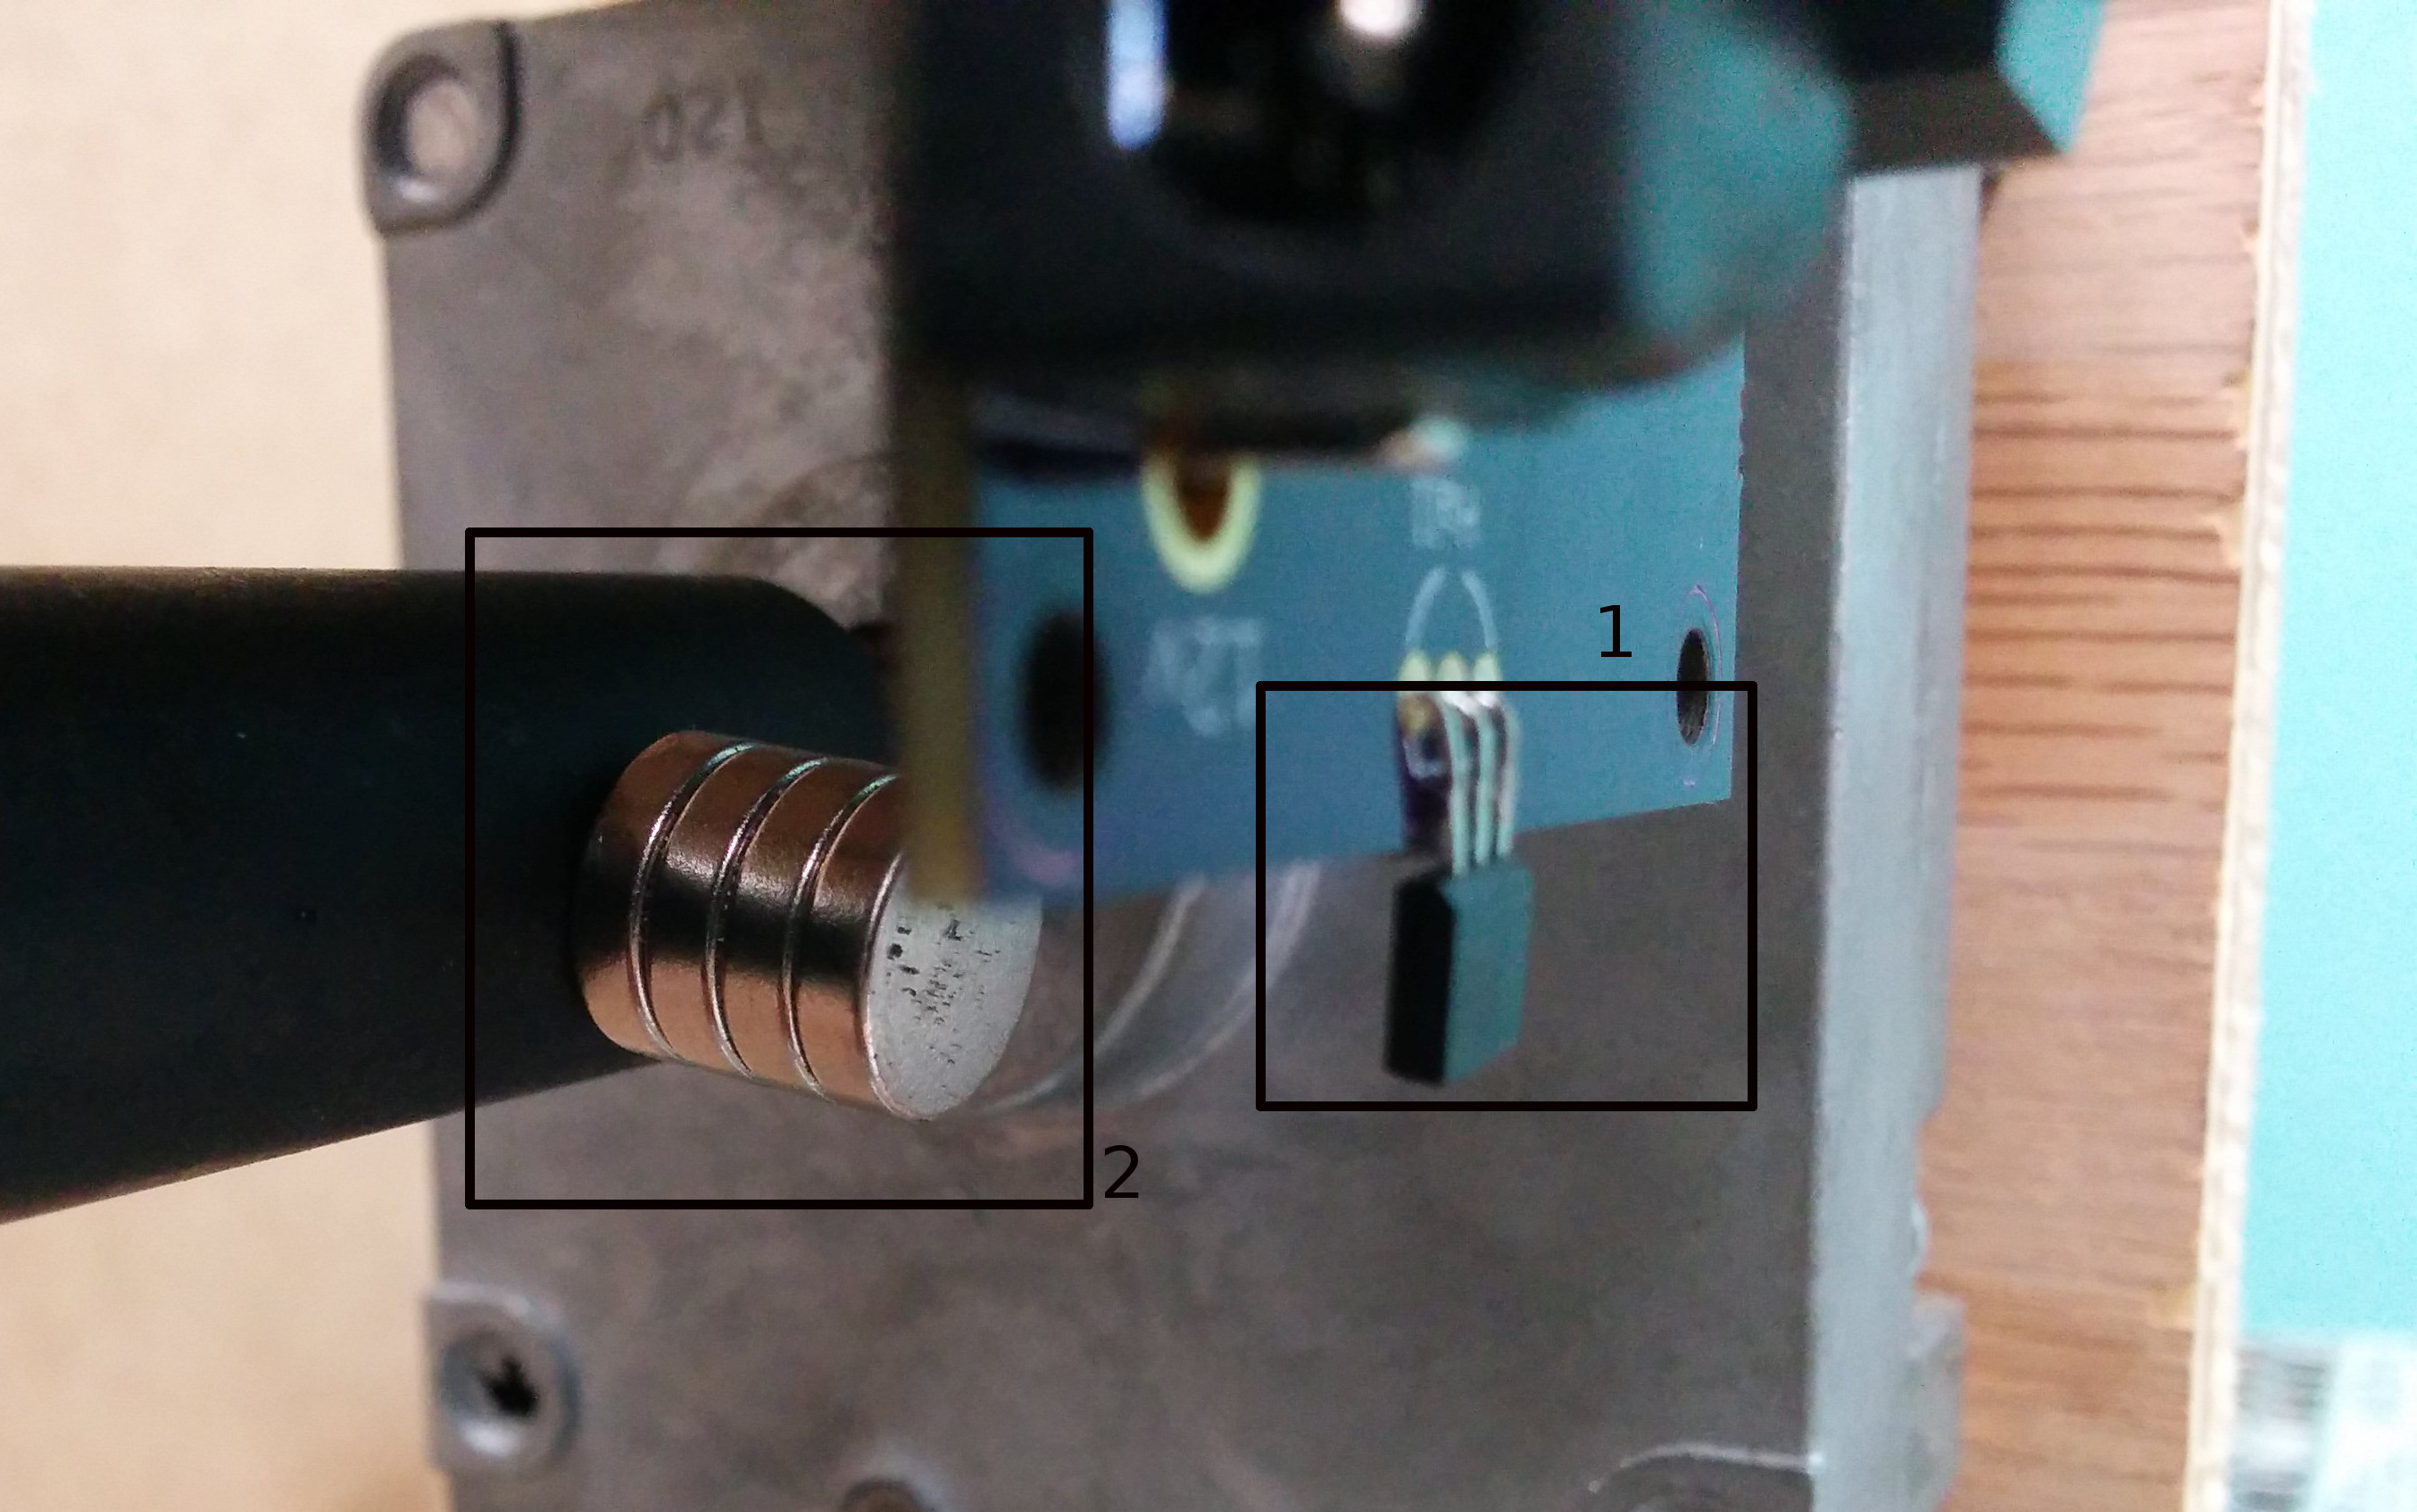
\includegraphics[width=0.8\textwidth]{images/producciones/20072015/IMG_20150721_110502.jpg}
    \caption[Encoder instalado en la filastruder.]{Encoder instalado en la filastruder. (1) Imanes que giran solidarios al husillo. (2) Sensor de Efecto Hall para detectar el paso de un campo magnético.}
    \label{fig:2007105-enc}
\end{figure}

Se extruye una cantidad de filamento sin medir el diámetro, tan sólo registrando la velocidad con la que gira el husillo y los datos proporcionados son los siguientesLa Figura \ref{fig:2007105-grafenc} muestra que la velocidad de giro no es constante, variando entre 1 y 2 RPM. 

\begin{figure}[H]
    \centering
    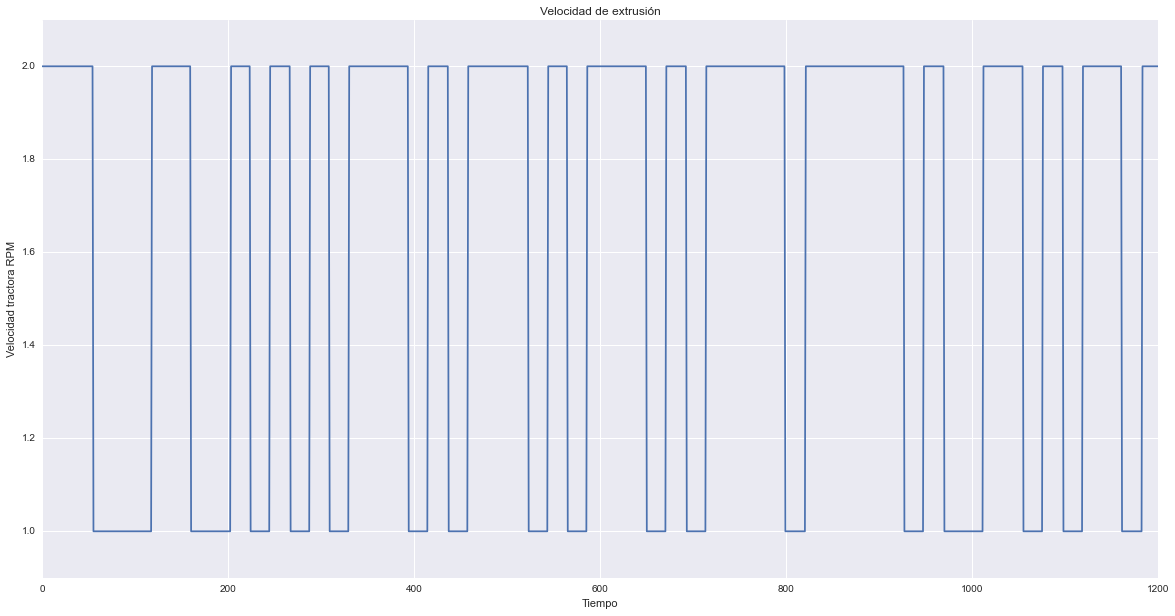
\includegraphics[width=0.99\textwidth]{images/producciones/20072015/RPM_tract.png}
    \caption[Velocidad de la extrusora]{Velocidad de la extrusora. Los datos reflejan como con un valor de referencia fijo de velocidad, esta sufre variaciones de las cuales no se tienen control.}
    \label{fig:2007105-grafenc}
\end{figure}

El motor que hace girar el husillo está conectado directamente a 12V y no se tienen ningún control sobre él. Además mecánicamente, el motor está conectado al husillo mediante una caja reductora, la cual no es posible cambiar.

Para solventar estos problemas, se van a tomar las siguientes medidas:

\begin{itemize}
    \item{Usar una mezcla de granza de PLA natural (70\%) con pellets reciclados de filamento (30\%) (ver Figura \ref{fig:2007105-mezc}). Se usará granza de PLA natural, el cual tiene una forma más redondeada que los pellets reciclados, haciendo más fácil el avance dentro del cañón. Se usa una mezcla con los pellets reciclados, ya que el sensor de diámetro que usamos, no funciona con filamento transparente, por ello, debemos tintar el filamento}
	    \begin{figure}[H]
		    \centering
		    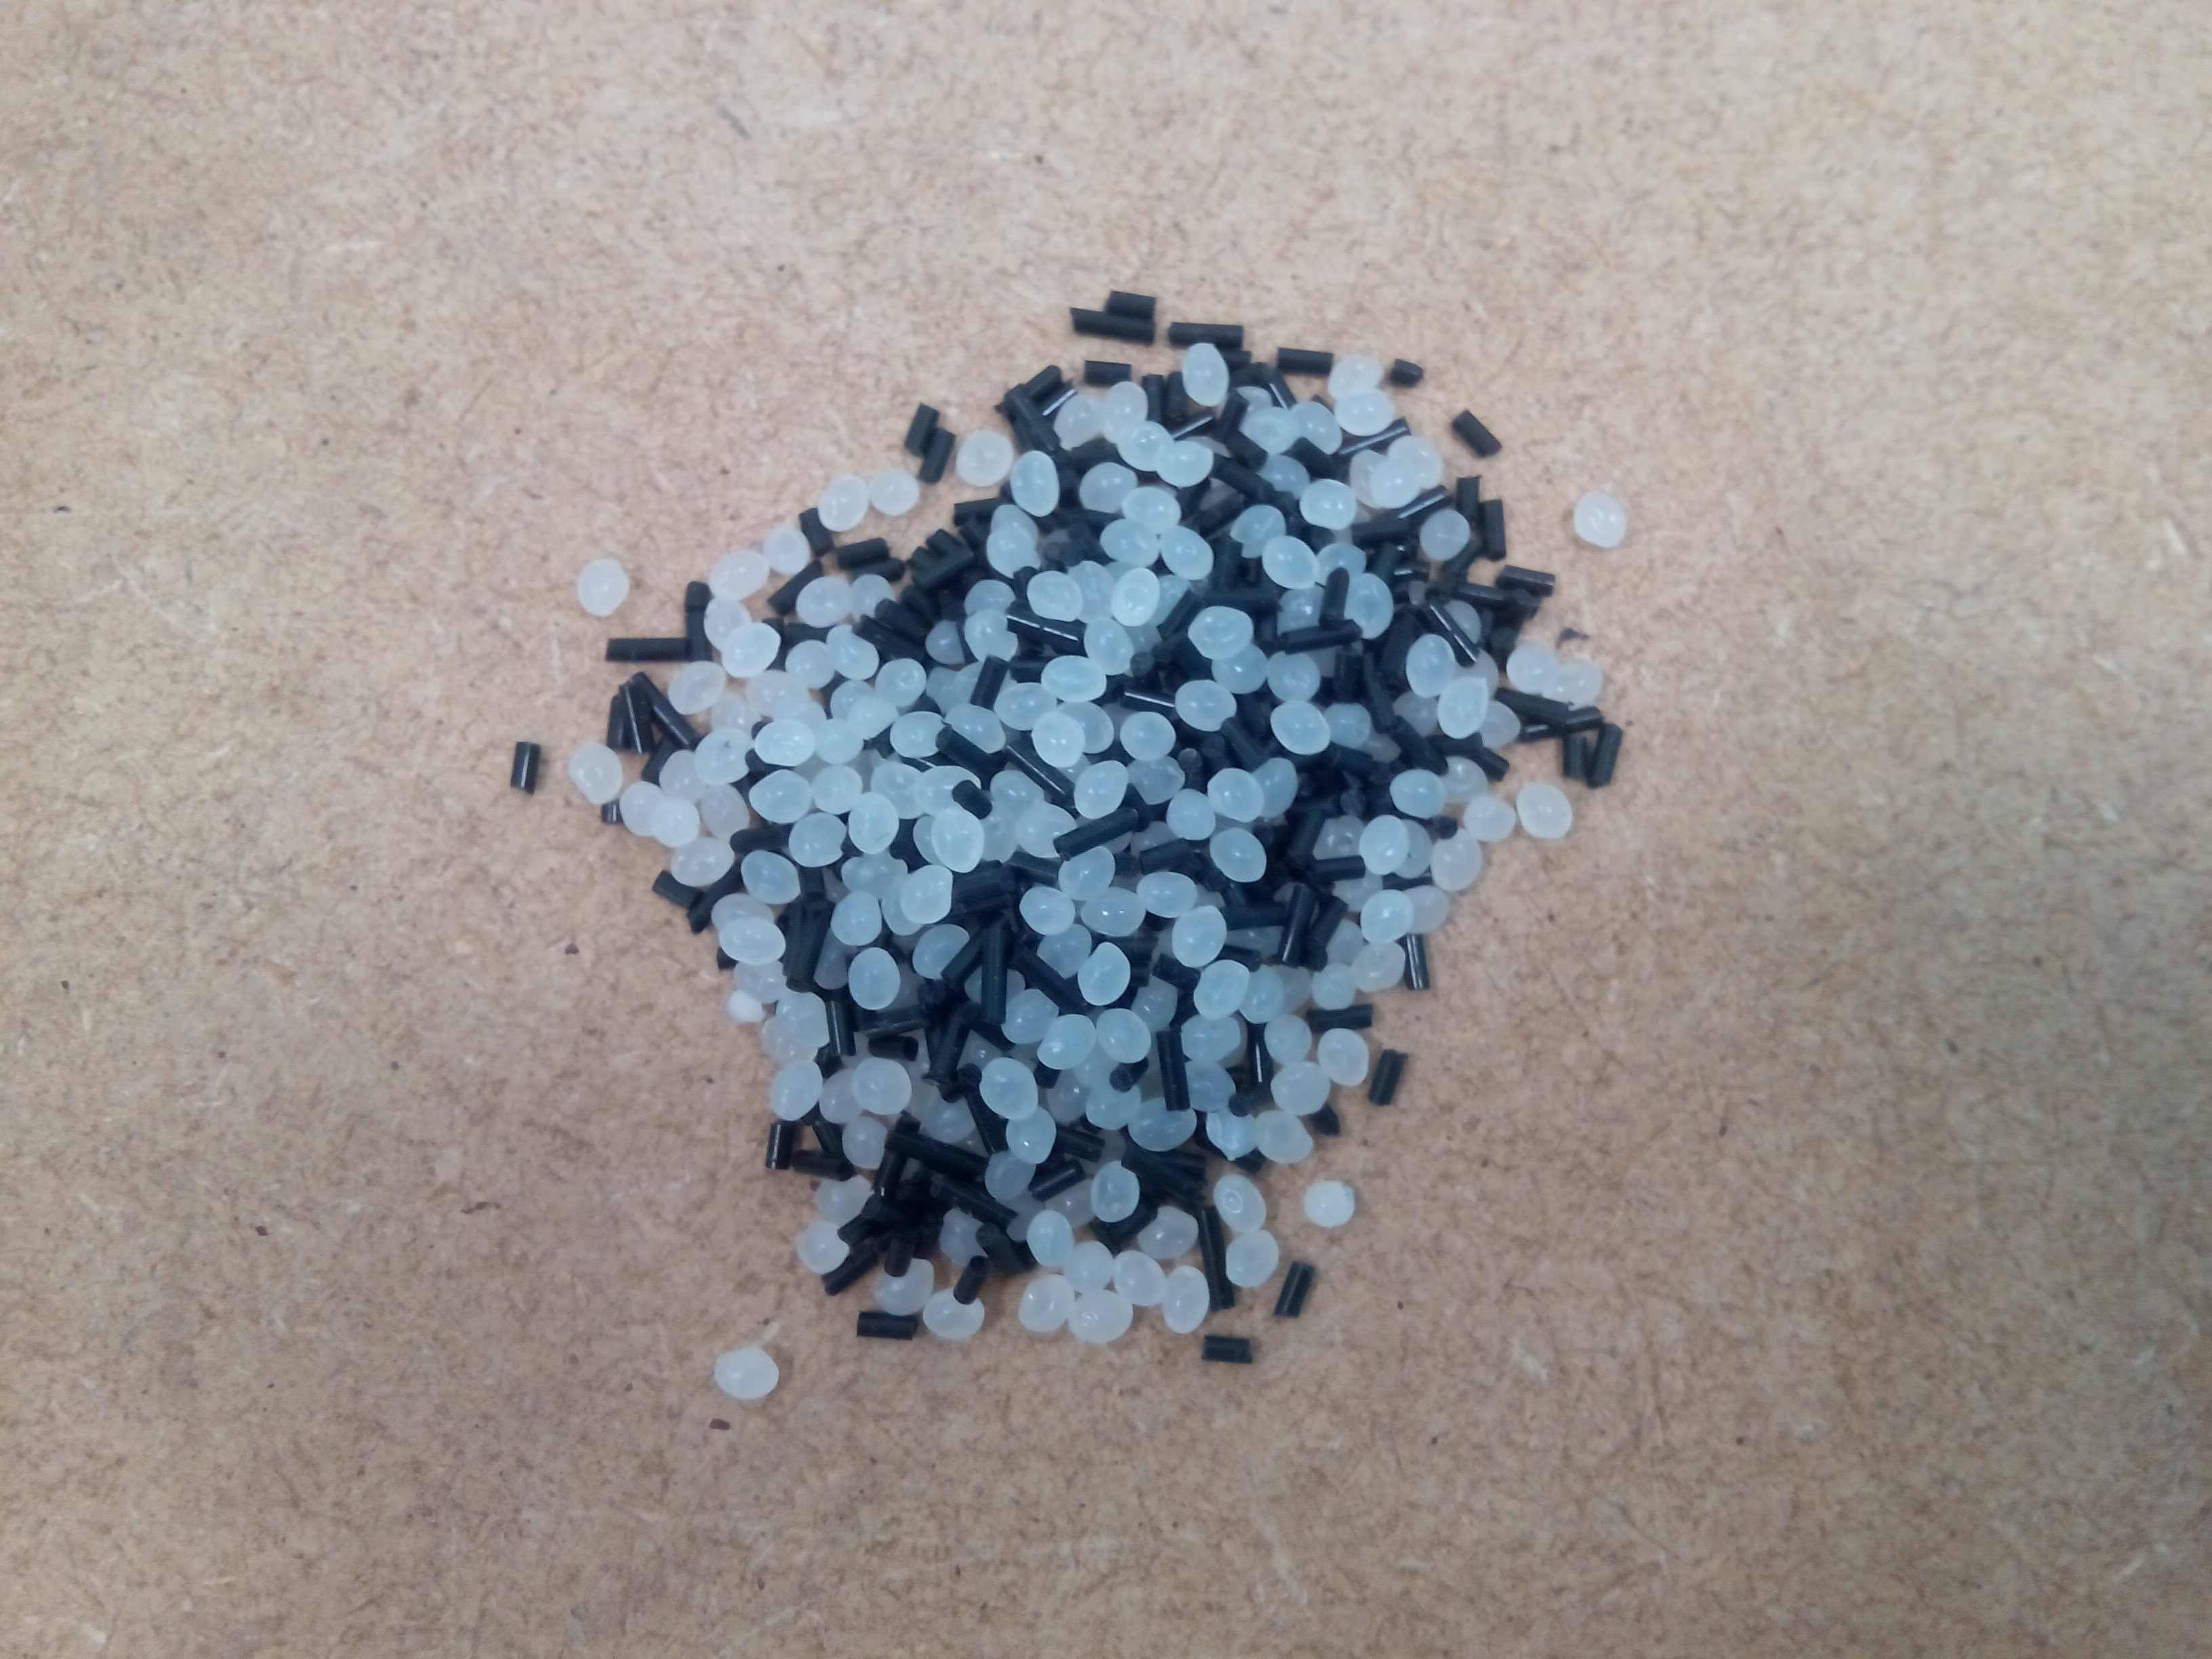
\includegraphics[width=0.4\textwidth]{images/producciones/20072015/IMG_20150903_155859.jpg}
		    \caption{Mezcla de granza con pellets reciclados.}
		    \label{fig:2007105-mezc}
		\end{figure}
    \item{Antes de hacer una producción de filamento, la granza de PLA que se vaya a usar, se va a secar en un horno a una temperatura de 80ºC durante, al menos, tres horas antes de la producción. Esto es debido a que si el PLA tiene un alto porcentaje de humedad, hará que la extrusión del material no sea el adecuado, afectando directamente en el acabado final.}
    \item{Se diseña una tolva de alimentación mayor, para que la capacidad de granza aumente, y se ejerza mayor presión a la entrada del extrusor, para que de ese modo, la alimentación de la granza sea lo más constante posible. El tamaño de almacenamiento máximo ha pasado de 42gr a 150gr (ver Figura \ref{fig:tolv_montaj}).}
\end{itemize}

\begin{figure}[H]
    \centering
        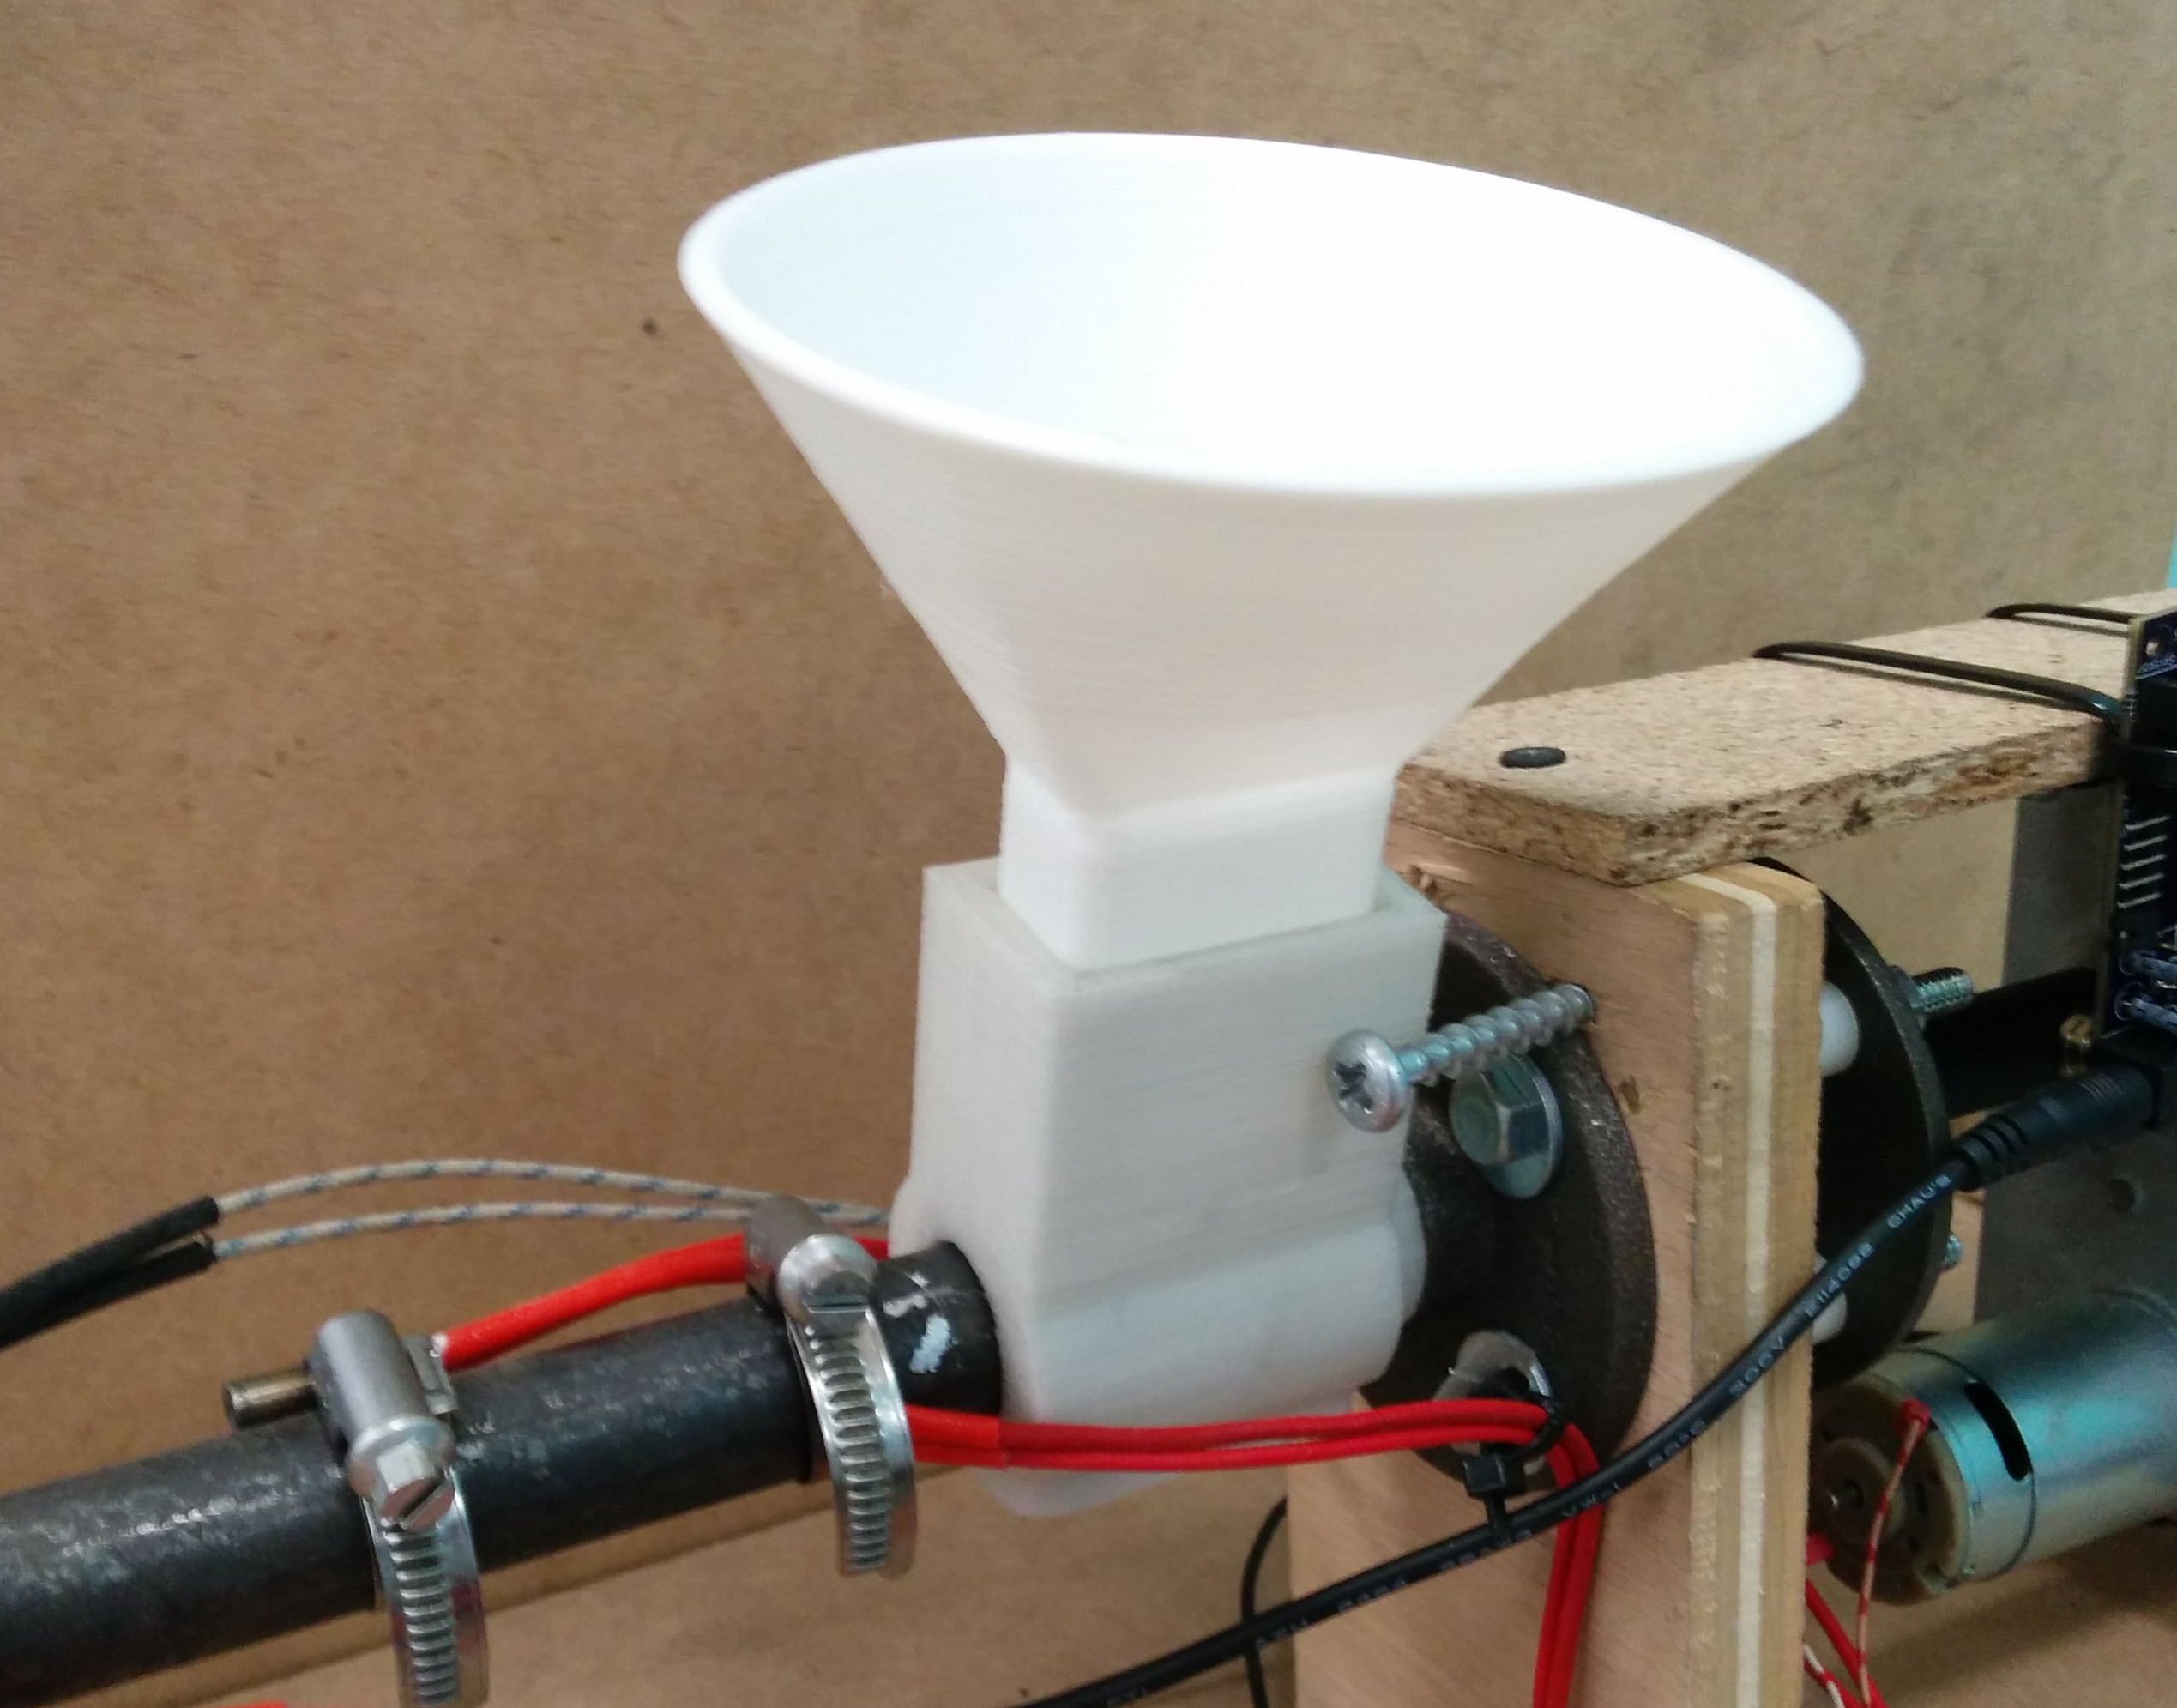
\includegraphics[width=0.5\linewidth]{images/producciones/20072015/IMG_20150721_121904.jpg}
        \caption[Diseño y montaje de una tolva de mayor capacidad.]{Diseño y montaje de una tolva de mayor capacidad.(1) Tolva que incluye de serie Filastruder, (2)La tolva que se ha diseñado añade mayor capacidad de pellets.}
        \label{fig:tolv_montaj}
\end{figure}

La Tabla \ref{tab:ensa_tolvas} muestra los resultados obtenidos en el ensayo:

\begin{table}[H]
    \centering
    \begin{tabular}{ccc}
                            & Tolva Grande & Tolva pequeña \\ \hline
        Muestras               & 2000  & 2000   \\
        Media (mm)          & 1.63     & 1.55      \\
        Desviación estandar & 0.14     & 0.15      \\
        Mínimo (mm)             & 1.02     & 0.01      \\
        Máximo (mm)             & 2.20     & 2.40     
    \end{tabular}
    \caption{Datos del ensayo con distintas tolvas}
    \label{tab:ensa_tolvas}
\end{table}

\begin{figure}[H]
    \centering
    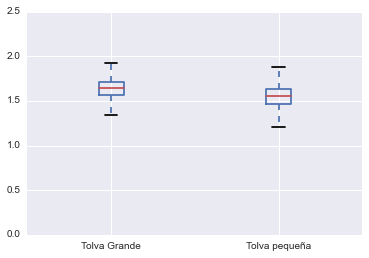
\includegraphics[width=0.8\textwidth]{images/producciones/22072015/output_6_1.png}
    \caption{Diagrama de cajas }
    \label{fig:22072015-boxplot}
\end{figure}

Como se ve en la Figura \ref{fig:22072015-boxplot}, en el que se representa la distribución de los datos, los datos obtenidos en el ensayo con la tolva grande, son algo más estables, por lo tanto, podemos confirmar, que las medidas tomadas para intentar mejorar la producción son acertadas, sin embargo, se sigue teniendo una variación y una desviación muy alta en el sistema, lo cual es un problema para intentar integrar un regulador del tipo PID. Por ello, se decide implementar un regulador experto para intentar controlar de forma más precisa el diámetro.


